\documentclass[a4paper,11pt]{article}
\usepackage[left=2.5cm, right=2.5cm, top=2cm, bottom=2.5cm]{geometry}
\usepackage{graphicx}
\usepackage{amssymb}
\usepackage{amsmath}
\usepackage{listings}
\usepackage{color} %red, green, blue, yellow, cyan, magenta, black, white
\definecolor{mygreen}{RGB}{28,172,0} % color values Red, Green, Blue
\definecolor{mylilas}{RGB}{170,55,241}

\begin{document}
\title{\LARGE{\textbf{ECEN 220 Lab 3}}}
\author{Niels Clayton \\300437590}
\date{}
\maketitle

\section*{Part 1: Matlab Fourier Transform $cos(w_0t)$}
\begin{center}
\fbox{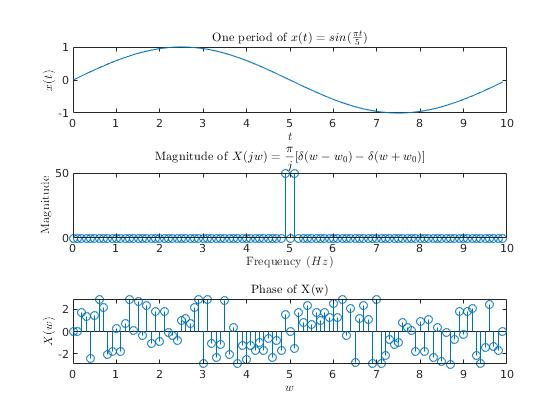
\includegraphics[scale=0.8]{q1.jpg}}
\end{center}

$cos(x)$ is an even function, this means that when taking the Fourier transform of it, the result should be purely real.  This means that we expect to see two peaks on the frequency spectrum of $w_0$ and $-w_0$, and for there to be zero phase. We do observe the expected peaks in frequency, however we don't observe the expected phases. This is do to floating point errors within a computer. When you manually look at the values of $X(jw)$ we can see that they all contain an imaginary component of the magnitude of $1\times 10^{-17}$. This imaginary component is almost non-existent, however it does still have a phase, leading to the noise seen.
\newpage

\section*{Part 2: Matlab Fourier Transform of other functions}

\begin{center}
\fbox{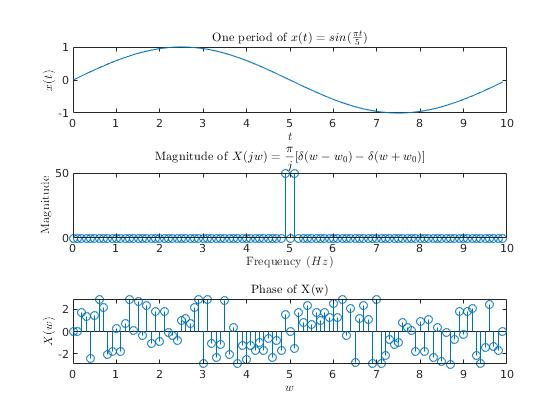
\includegraphics[scale=0.8]{sine.jpg}}
\end{center}

\begin{center}
\fbox{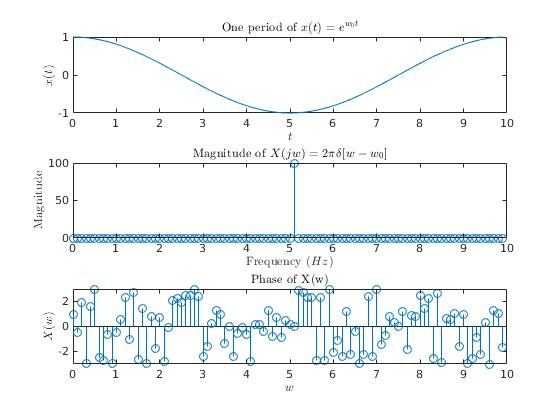
\includegraphics[scale=0.8]{e.jpg}}
\end{center}

\begin{center}
\fbox{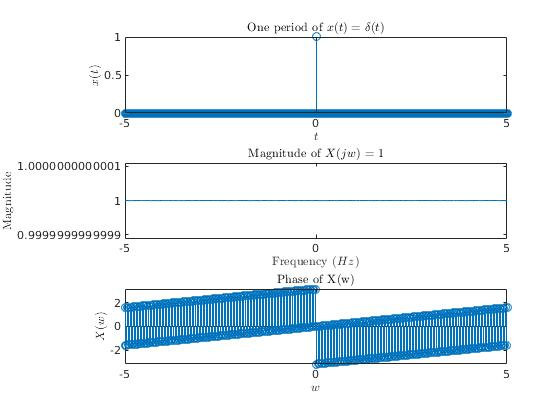
\includegraphics[scale=0.8]{delta.jpg}}
\end{center}

\begin{center}
\fbox{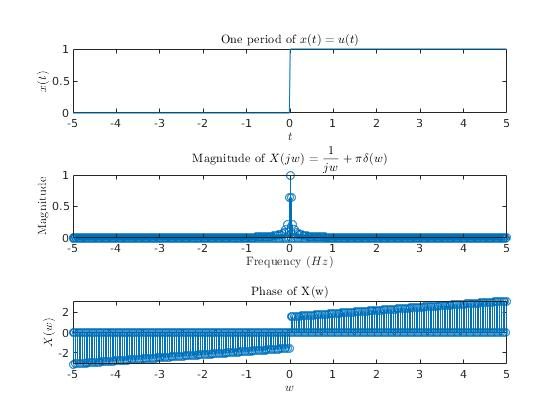
\includegraphics[scale=0.8]{u.jpg}}
\end{center}

\begin{center}
\fbox{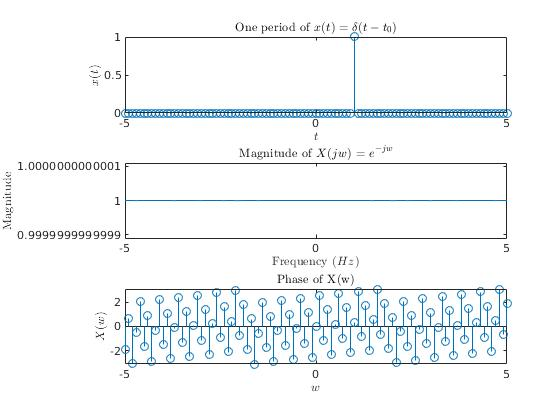
\includegraphics[scale=0.8]{deltashift.jpg}}
\end{center}

\begin{center}
\fbox{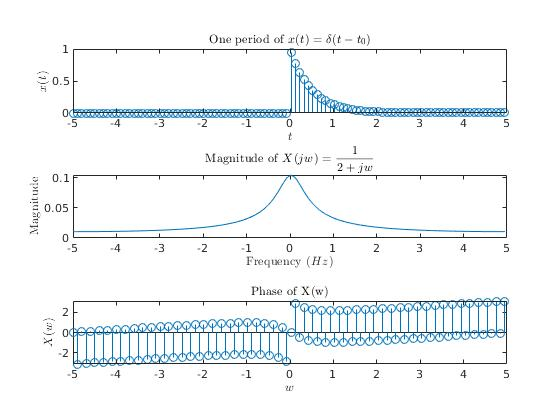
\includegraphics[scale=0.8]{e2.jpg}}
\end{center}

\begin{center}
\fbox{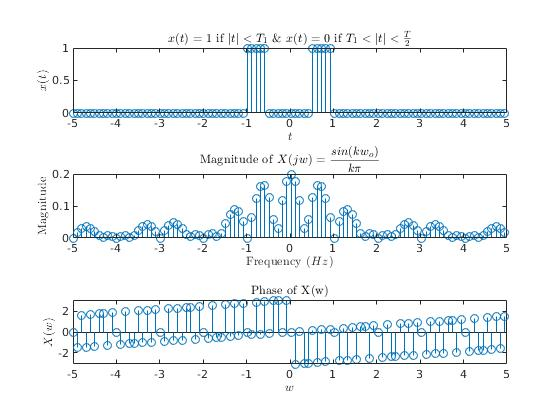
\includegraphics[scale=0.8]{sinc.jpg}}
\end{center}

\newpage



\lstset{language=Matlab,%
    %basicstyle=\color{red},
    breaklines=true,%
    morekeywords={matlab2tikz},
    keywordstyle=\color{blue},%
    morekeywords=[2]{1}, keywordstyle=[2]{\color{black}},
    identifierstyle=\color{black},%
    stringstyle=\color{mylilas},
    commentstyle=\color{mygreen},%
    showstringspaces=false,%without this there will be a symbol in the places where there is a space
    numbers=left,%
    numberstyle={\tiny \color{black}},% size of the numbers
    numbersep=9pt, % this defines how far the numbers are from the text
    emph=[1]{for,end,break},emphstyle=[1]\color{red}, %some words to emphasise
    %emph=[2]{word1,word2}, emphstyle=[2]{style},    
}
\section*{Matlab Code}

\lstinputlisting{lab_3.m}

\end{document}
